\section{Funcionamiento}
La interfaz del servidor es sencilla.

\begin{figure}[H]
	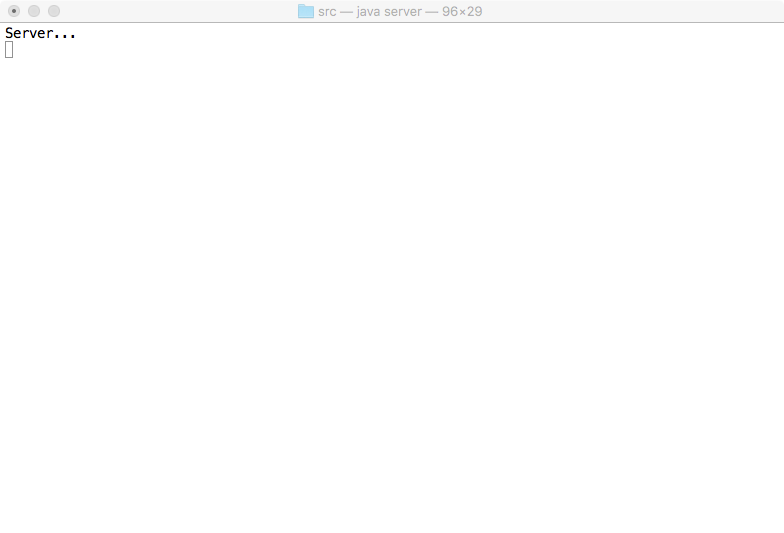
\includegraphics[scale=0.65]{./Imagenes/server1.png}
\end{figure}



% -----------------------------------


\subsection{Cliente}
Cada usuario tiene un terminal para el Writer y otro para el Printer.

\begin{figure}[H]
	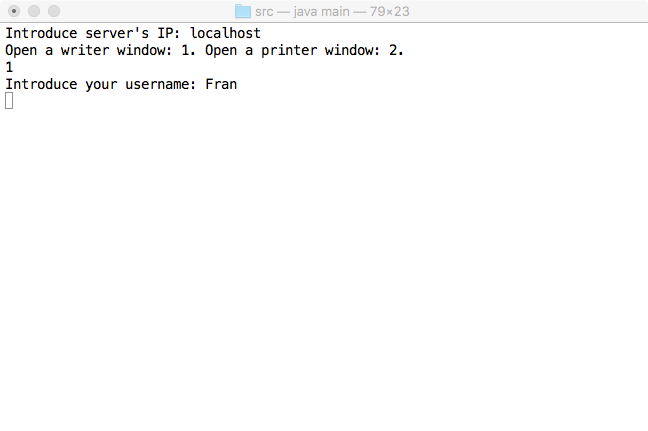
\includegraphics[scale=0.65]{./Imagenes/franwriter1.png}
	\caption{Fran writer}
\end{figure}

\vspace{0.1cm}

\begin{figure}[H]
	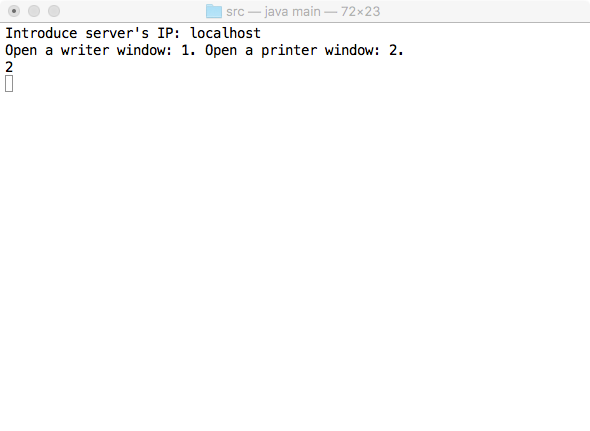
\includegraphics[scale=0.65]{./Imagenes/franprinter1.png}
	\caption{Fran printer}
\end{figure}

\vspace{0.1cm}

\begin{figure}[H]
	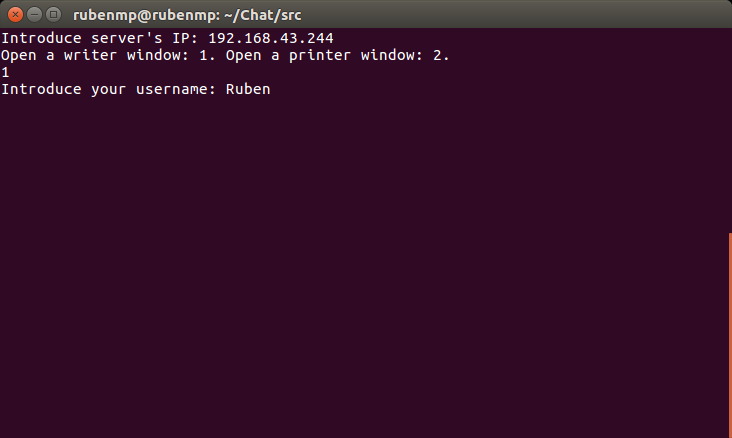
\includegraphics[scale=0.65]{./Imagenes/rubenwriter1.png}
	\caption{Ruben writer}
\end{figure}

\vspace{0.1cm}

\begin{figure}[H]
	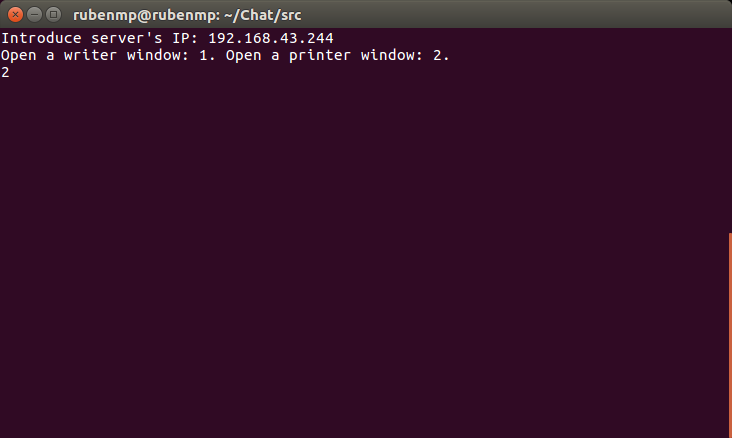
\includegraphics[scale=0.65]{./Imagenes/rubenprinter1.png}
	\caption{Ruben printer}
\end{figure}


\subsection{Escribir mensajes}
Ahora procedemos a escribir mensajes desde ambos ordenadores.

\begin{figure}[H]
	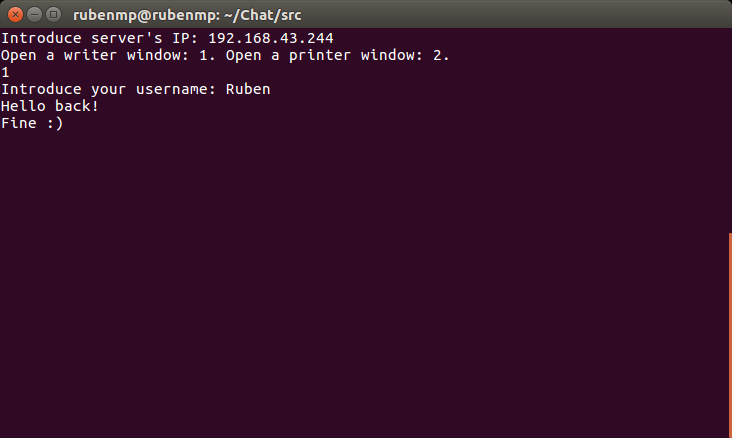
\includegraphics[scale=0.65]{./Imagenes/rubenwriter2.png}
	\caption{Ruben escribiendo}
\end{figure}

\vspace{0.1cm}

\begin{figure}[H]
	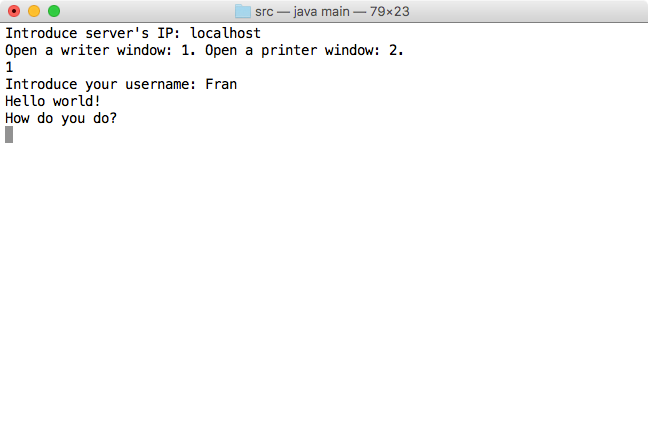
\includegraphics[scale=0.65]{./Imagenes/franwriter2.png}
	\caption{Fran escribiendo}
\end{figure}

Comprobamos que funciona

\begin{figure}[H]
	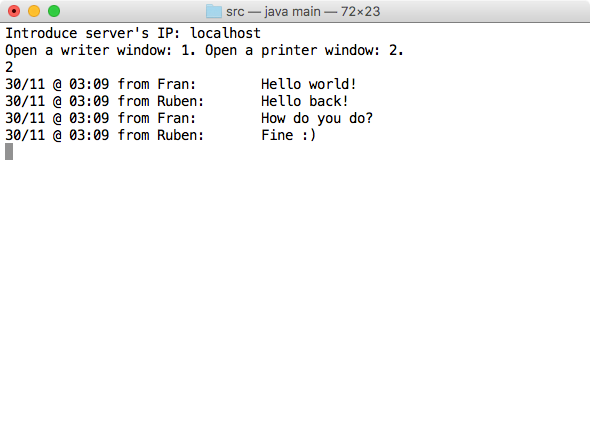
\includegraphics[scale=0.65]{./Imagenes/franprinter2.png}
	\caption{Fran recibiendo}
\end{figure}

\vspace{0.1cm}

\begin{figure}[H]
	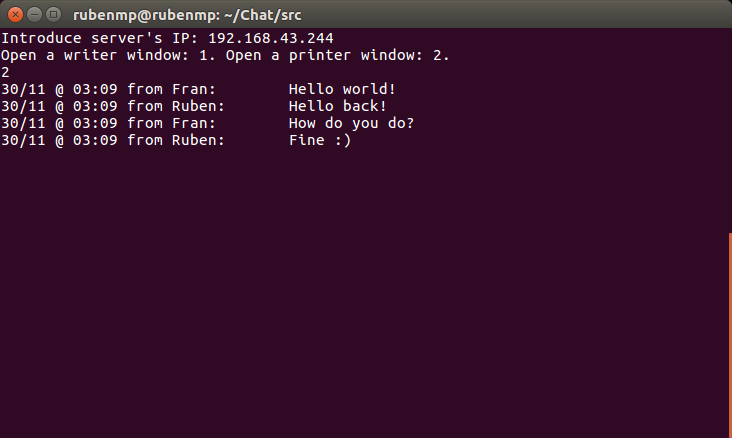
\includegraphics[scale=0.65]{./Imagenes/rubenprinter2.png}
	\caption{Ruben escribiendo}
\end{figure}


